\documentclass[12pt]{article}
\usepackage{xcolor}
\usepackage[latin]{babel}
\usepackage[utf8]{inputenc}
\usepackage[T1]{fontenc}
\usepackage{amsmath}
\usepackage{amsfonts}
\usepackage{amssymb}
\usepackage[version=4]{mhchem}
\usepackage{stmaryrd}
\linespread{1.5}
\setlength{\parindent}{0pt}
\usepackage{listings}
\usepackage{xcolor}
\usepackage{algorithm}
\usepackage{algpseudocode}
\usepackage{tikz}
\usepackage{pifont}
\usepackage{tikz}
\usetikzlibrary{positioning}  
\begin{document}

$\text{Q}_{1}$

a.

PF:

1. Assume each of the clusters \(\{a,b\}, \{e\}, \{d,c,i,f,g,h\}\) is a tree.

2. Assume \(T \subseteq T_{\min}\) for some MST \(T_{\min}\).

As \(\{a, b\} \neq \{d, c, i, f, j\}\), we add \((a, h)\) to $T$.

WTP:

1. Each of the clusters \(\{a,b,d,c,i,f,g,h\}, \{e\}\) is a tree.

2. Assume \(T = \{ (g,h), (c,i), (f,g), (c,f), (a,b), (c,d) , (a, h)\}\subseteq T_{\min}\) for some MST \(T_{\min}\).

Consider $\{a , b\}$ and $\{ d,c,i,f,g,h \}$ in our assumption 

we have $\{a , b\}$ and $\{ d,c,i,f,g,h \}$ two trees

$\Rightarrow 1^{\circ}$ no circle in $\{a ,b\}$ and $\{ d,c,i,f,g,h \}$ ($*$)

$2^{\circ}$ $\{a , b\}$ are connected with each other and $\{ d,c,i,f,g,h \}$ are connected with each other

$\because\{a, b\} \neq \{ d,c,i,f,g,h \}$

$\therefore(a, h) $ is added to $T$

$\Rightarrow\{a,b,d,c,i,f,g,h\}$ are connected with each other (1) 

suppose there is a circle in $\{a,b,d,c,i,f,g,h\}$

by ($*$)

there are at least 2 paths that connect $\{a,b\}$ and $\{d,c,i,f,g,h \}$

$\because(a,h)$ is a path (edge) that connects $\{a,b\}$ and $\{d,c,i,f,g,h \}$

so before adding $(a, h)$. there is still a path that connects $\{a,b\}$ and $\{d,c,i,f,g,h \}$

then after adding the path. $\{a, b\}$ and $\{d,c,i,f,g,h \}$ should already be merged together before adding $(a,b)$

$\Rightarrow$ this is a contradiction

$\Rightarrow$ The supposition is false and there is no circle in $\{a,b,d,c,i,f,g,h \}$ (2) 

By (1) and (2).

$\{a,b,d,c,i,f,g,h \}$ is a tree and so is $\{e\}$

Call the set $T$ before processing $(a,h,8)$ $T_1$ and the set $T$ after processing $(a,h,8)$ $T_2$

we have $T_1 \subseteq T_{\min }$ for some MST $T_{\min }$, let's call the $T_{\min }$ ``$T_{\text {mink }}$''

if $(a, h) \in T_{\text {mink }}$, then $T_2=T_1 \cup\{(a , h)\} \subseteq T_{\text {mink }}$

$\Rightarrow T_2 \subseteq T_{\min }$ for some MST $T_{\text {min }}$

if $(a, h) \not\in T_{\text {mink }}$

$\Rightarrow$ divide vertices into two sets $S$ and $V-S$

$S=\{a, b\}$

$V-S=\{d, c , i, f, g, h, e\}$

there is no $T_1$ edge between $S$ and $V-S$

in $T_{\text {mink }}$, there exists a unique path that connects $a$ and $u$, and there is an edge on this path that connects $S$ and $V-S$ 

In the graph, we have such edges $(a,h)$ and $(b,c)$

$\because(a, h) \not\in T_{\text {mink }}$ 

$\therefore(b,c) \in T_{\text {mink }}$

$\because$ weight $(a , h)=$ weight $( b, c)=8$

$\therefore T_{\text {mink }}{ }^{\prime}=T_{\text {mink }}-\{(b ,c)\}+\{(a,h)\}$ has the same weight as $T_{\text {mink }}$

$T_{\text {mink }}$ is disconnected after removing $(b, c)$, but reconnected after adding $(a,h)$

In $T_{\text {mink }}$, there is no circle.

So there is no circle in $T_{\text {mink }}{ }^{\prime}$ as we use one unique edge to link these two parts: $\{a ,b\}$ and $\left\{h, g, f, c, i, d, e\right\}$.

$\Rightarrow$ $T_{\text {mink }}{ }^{\prime}$ is a MST

$\because T_2 \subseteq T_{\text {mink }}{ }^{\prime}$

$\therefore T=\left\{(g, h),(c, i),(f,g),(c,f),(a,b),(c, d),(a,h)\right\} \subseteq T_{\text {min }}$ for some MST $T_{\text {min }}$

QED.

b.

PF:

Assume $T$ contains vertices $a, b$ and $P Q$ contains vertices $c, d, e ,f, g, h, i$.

Assume for each $v$ in $P Q$, priority $(v)=$ minimum weight of any edge between $v$ and $T$.

Assume $T \subseteq T_{\text {min }}$ for some MST $T_{\text {min }}$

WTP.

After de-queuing $h$,

$T$ contains $a, b, h$ and $P Q$ contains $c, d, e, f, g, i$

for each $v$ in $P Q$, priority $(v)=$ minimum weight of any edge between $V$ and $T$ 

$T \subseteq T_{\text {min }}$ for some MST $T_{\text {min }}$

After de-queuing $h,(a, h)$ is added to $T$

so $T$ has $h$ and $P Q$ only lose $h$

$\Rightarrow T$ contains $a, b, h$ and $P Q$ contains $c, d, e, f, g, i$

As $T$ is only extended a vertex $h$, the vertices in $P Q$ whose priorities are charged can only be the adjacency of $h$, as they have a new edge to the new $T$.

By the algorithm and the graph, only $i$ and $g$ need to update their priority and they will still be the minimum weight of any edge between $i || g$ and new $T$ (``the decrease-priority ()'' lets $g$ and $i$ always choose the minimum weight).

From our assumption, $c, d, e, f$ have the priorities that are the minimum weight of any edge between $c||d||e||f$ and old $T$.

The dequeue operation doesn't affect $c||d||e||f$:

1. The new T's new edge $(a, h)$ still doesn't generate a new edge to $c||d||e||f$

2. Priorities of $c||d||e||f$ aren't changed.

$\Rightarrow$ $c||d||e||f$ have priorities that are equal to minimum weight of any edge between $c||d||e||f$ and new $T$. (4)

By (3) (4). for each $v$ in new $P Q$, priority $(v)=$ minimum weight of any edge between $v$ and new $T$

Call $T$ before de-queuing $h$ be $T_3, T$ after de-queuing $h$ be $T_4$.

We have $T_3 \subseteq T_{\min }$ for some MST.

Call the $T_{\text {min }}$ be $T_{\text {minkb}}$.

If $(a, h) \in T_{\text {minkb }}$, then $T_4=T_3 \cup\{(a, h)\} \subseteq T_{\text {minkb }}$.

$\Rightarrow$ After de-queuing $h, T \subseteq T_{\text {min }}$ for some MST $T_{\text {min }}$ 

If $(a, h) \not\in T_{\text {minkb}}$, 

then divide $V$ into $\{a ,b\}$, and $\{h, i, c, d, e, f, g\}$ two parts.

There is a unique path in $T_{\text {minkb}}$ that connects $a$ and $h$, and there is a unique edge that connects these two parts. 

In the given graph, they are $(a,h)$ and $(b,c)$

$\because(a, h) \notin T_{\text {minkb }} $

$\therefore$ The unique edge is $(b, c)$

$\because$ weight $(b,c)=$ weight $(a,h)=8$

$\therefore$  $T_{\text {minkb }}{}^{\prime}=T_{\text {minkb }}-\{(b, c)\}+\{(a , h)\}$ has the same weight as $T_{\text {minkb }}$

$T_{\text {minkb }}$ is disconnected after removing $(b,c)$ and reconnected after adding $(a, h)$ with no circles produced.

$T_{\text {minkb }}{}^{\prime}$ is a MST

$T_4=T_3 \cup\{(a, h)\} \subseteq T_{\text {minkb }}{}^{\prime}$

$\therefore$ After de-queuing $h, T\subseteq T_{\text {min }}$  for some MST $T_{\text {min }}$

QED.

\newpage
$\text{Q}_{2}$

a.

PF:

Consider two cases:

$1^{\circ}$ The graph has no negative weights

Then by line 1: minimum\_weight $>0$

$\therefore c=0$

$\therefore \forall e\in E$ , weight $'(e)=$ weight (e $)$

$\Rightarrow$ line 5 is actually using the Prim algorithm on the given graph directly.

$\Rightarrow$ the output of this new algorithm is the MST of both the given graph with modified weight and the given graph with original weight.

$2^{\circ}$ The graph has negative edges

$\Rightarrow$ minimum\_weight $<0$

$\Rightarrow c \geq$ $-$minimum\_weight $>0$

$\Rightarrow$ for an arbitrary edge $(u,v)$ in $E$

weight ${ }^{\prime}(u,  v)=$ weight $(u,  v)+c \geqslant$ minimum\_weight $+(-$minimum\_weight $)=0$

$\Rightarrow \forall e \in E$, weight ${ }^{\prime}(e) \geqslant 0$

After line 5,

according to the lecture, a MST of the given graph with modified weights is produced.

Let's suppose the MST be $T_{\text {min }}^{\prime}=\left\{e_1^{\prime},  e_2^{\prime}\ldots e_t^{\prime}\right\} \subseteq E \quad(t=|V|-1)$ \ding{172}

WTP: $T'_{min}$ is also a MST in the given graph with original weights 

As $T'_{min}$ is a MST in the modified graph,

it connects all the vertices of the modified graph and no circle 

$\because$ The given graph with modified weights has the same $V$ and $E$ as the given graph with original weights

$\Rightarrow$ $T'_{min}$ connects all the vertices in the original given graph and no circle $(*)$

Now we need to show that $T'{min}$ is also the spanning tree with minimum weight of the original graph.

Suppose $T'_{min}$ in the original-weight graph is not the one with minimum weight.

$\Rightarrow$ there exists a MST $T_{min}$ in the original graph whose total weight is smaller than $T'_{min}$'s.

let $T_{\min }=\left\{e_1, e_2 \ldots e_m\right\} (m=|V|-1)$

by \ding{172}

$m=t$

$\therefore T_{\min }=\{e_1, e_2 \ldots e_t\}$

$ W\left(T_{\text {min }}\right)=\sum\limits_{i=1}^t \text { weight }\left(e_i\right)<\sum\limits_{i=1}^t \text { weight }\left(e_i^{\prime}\right)=W\left(T_{\text {min }}^{\prime}\right) $

$\begin{aligned}
 \Rightarrow W^{\prime}\left(T_{\text {min }}^{\prime}\right)=\sum\limits_{i=1}^{ t} \text {weight}^{\prime}\left(e_i^{\prime}\right)&=\sum\limits_{i=1}^{ t} \text ({weight }\left(e_i^{\prime}\right)+c)\\
&=\sum\limits_{i=1}^{ t} \text {weight }\left(e_i^{\prime}\right)+tc\\
& =W\left(T_{\text {min }}^{\prime}\right)+t c \\
& >W\left(T_{\text {min }}\right)+t c \\
& =\sum\limits_{i=1}^t \text { weight }\left(e_i\right)+t c \\
& =\sum\limits_{i=1}^t \text ({ weight }\left(e_i\right)+c) \\
& =\sum\limits_{i=1}^t  \text { weight }^{\prime}\left(e_i\right) \\
& =W^{\prime}\left(T_{\text {min }}\right)
\end{aligned}
$

$\because T_{\min }^{\prime}$ is a MST in the modified-weight graph

$\therefore W^{\prime}\left(T_{\text {min }}^{\prime}\right) \leqslant W^{\prime}\left(T_{\text {min }}\right)$

$\Rightarrow$ There is a contradiction.

$\Rightarrow$ Our supposition is false

$\therefore $ $T'_{min}$ has the minimum weight in the original given graph
(\#)

By (*) and (\#),

$T'_{min}$ is also a MST in the original given graph

$\Rightarrow$ The new algorithm outputs an MST.

QED.

b.

We can't get the shortest path to some vertices, as there may be no shortest path to some vertices in a graph with negative weights (no lower bound for the weights of some paths) 

Consider this graph: 
\begin{center}
    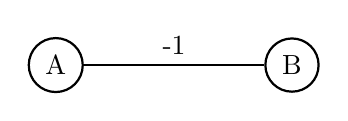
\begin{tikzpicture}
        \node[circle,draw,thick] (A) at (0,0) {A};
        \node[circle,draw,thick] (B) at (3,0) {B};
        \draw[thick] (A) -- (B) node[midway,above] {-1};
    \end{tikzpicture}
\end{center}

As we do not need the path to be simple, then the path from $A$ to $B$ can be:

$\{A, B\} \text { weight }=-1 $

$ \{A,  B, A, B\} \text { weight }=-3 $

$ \{A, B, A, B, A, B\} \text {  weight }=-5$

$ \underbrace{\{A,  B,  A,  B,..., A,  B\}}_{n ``A, B"} \text { weight }=-2 n+1$

we can get infinite paths by walking back and forth between $A$ and $B\quad  n$ times $(n \in N)$ and stop at $B$, the weights of those paths will decrease as $n$ increase and will never come to an end as $n$ has no upper bound. (i.e. the weight can be $-\infty$ )

$\Rightarrow$ then we can't get the shortest path from $A$ to $B$

c. Disprove,

Consider this graph:
\begin{center}
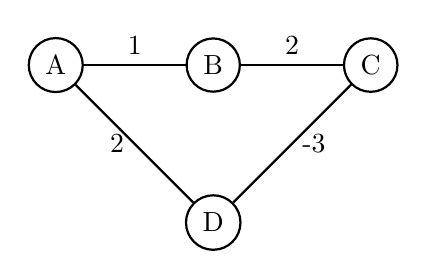
\begin{tikzpicture}
    \node [circle,draw,thick] (A) at (0,0) {A};
    \node [circle,draw,thick] (B) at (2,0) {B};
    \node [circle,draw,thick] (C) at (4,0) {C};
    \node [circle,draw,thick] (D) at (2,-2) {D};
    \draw[thick] (A) -- (B) node[midway,above] {1};
    \draw[thick] (B) -- (C) node[midway,above] {2};
    \draw[thick] (A) -- (D) node[midway,left] {2};
    \draw[thick] (C) -- (D) node[midway,right] {-3};
\end{tikzpicture}
\end{center}

if we set $A$ be the starting point, then by Dijkstra's algorithm:

\ding{172}

$\begin{array}{lllll}
A & B & C & D & \text{Distance tree: } \{\}\\
0 & \infty & \infty & \infty
\end{array}$

\ding{173}

$\begin{array}{lllll}
B & D & C & \text{Distance tree: } \{\}\\
1 & 2 & \infty \\
A & A &
\end{array}$

\ding{174}

$\begin{array}{lllll}
D & C & \text{Distance tree: } \{(A, B, 1)\}\\
2 & 3 &  \\
A & B &
\end{array}$

\ding{175}

$\begin{array}{lllll}
C &  & \text{Distance tree: } \{(A, B, 1), (A, D, 2)\}\\
-1 &  &  \\
D &  &
\end{array}$

\ding{176} Distance tree: $\{(A, B, 1) , (A, D, 2) , (D, C,-1)\}$

$\Rightarrow \delta(D)=2$

but in our graph $\delta(D)$ should be $1+2-3=0$ 

$0<2$

$\therefore$ We fail to find the single-source shortest simple path from $A$ to $D$ with Dijkstra's algorithm.

This is because if we want to have $\delta_{\text {fin}}(D)=0$, we need to dequeue $A ,  B ,  C$ first. But in the algorithm $p(C)=\delta_{\text {fin}}(C)=3>p(D)$ $=\delta_{\text {fin}}(D)=2$. This means we have to dequeue $D$ first in the algorithm and that makes our algorithm fail to find the single-source shortest simple path from $A$ to $D$.

QED.

d. Disprove 

Consider the graph
\begin{center}
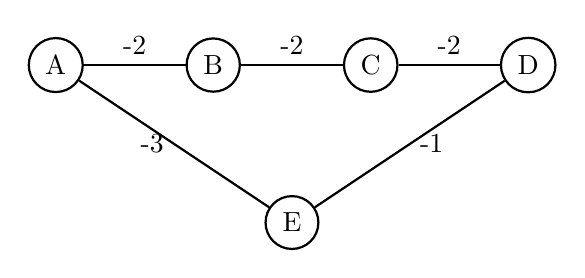
\begin{tikzpicture}
    \node [circle,draw,thick] (A) at (0,0) {A};
    \node [circle,draw,thick] (B) at (2,0) {B};
    \node [circle,draw,thick] (C) at (4,0) {C};
    \node [circle,draw,thick] (D) at (6,0) {D};
    \node [circle,draw,thick] (E) at (3,-2) {E};
    \draw[thick] (A) -- (B) node[midway,above] {-2};
    \draw[thick] (B) -- (C) node[midway,above] {-2};
    \draw[thick] (C) -- (D) node[midway,above] {-2};
    \draw[thick] (A) -- (E) node[midway,left] {-3};
    \draw[thick] (D) -- (E) node[midway,right] {-1};
\end{tikzpicture}
\end{center}

the single-source shortest simple path from $A$ to $D$ is $\{A ,  B ,  C ,  D\}$ weight $=-6$

but by the modified Dijkstra's algorithm:

The graph will become
\begin{center}
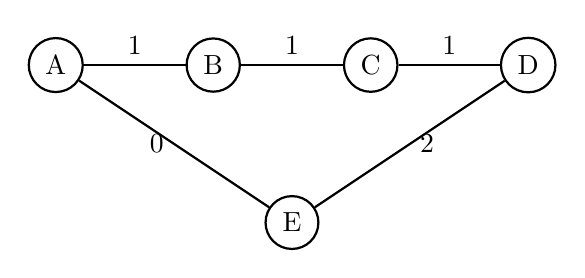
\begin{tikzpicture}
    \node [circle,draw,thick] (A) at (0,0) {A};
    \node [circle,draw,thick] (B) at (2,0) {B};
    \node [circle,draw,thick] (C) at (4,0) {C};
    \node [circle,draw,thick] (D) at (6,0) {D};
    \node [circle,draw,thick] (E) at (3,-2) {E};
    \draw[thick] (A) -- (B) node[midway,above] {1};
    \draw[thick] (B) -- (C) node[midway,above] {1};
    \draw[thick] (C) -- (D) node[midway,above] {1};
    \draw[thick] (A) -- (E) node[midway,left] {0};
    \draw[thick] (D) -- (E) node[midway,right] {2};
\end{tikzpicture}
\end{center}
    
After line 5 in modified Dijkstra's algorithm:

In the single-source shortest simple paths that output by line 5,
the shortest path from $A$ to $D$ will be $\{A, E, D\}$ with weight $=2$ 

Now put it back to the original graph.

$\{A, E, D\}$ is weighted -4 , which is larger than the actual shortest simple path from $A$ to $D$ $\{A, B, C, D\}$ with weight $=-6$.

$\Rightarrow$ The new algorithm fails to output the right shortest single path for $A$ to $D$.

$\Rightarrow$ the new algorithm doesn't output all the single-source shortest simple paths

$\Rightarrow$ so disprove the statement.

QED.

\newpage
$\text{Q}_{3}$

a.

Disprove:

Consider the graph:
\begin{center}
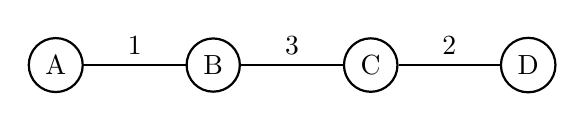
\begin{tikzpicture}
    \node [circle,draw,thick] (A) at (0,0) {A};
    \node [circle,draw,thick] (B) at (2,0) {B};
    \node [circle,draw,thick] (C) at (4,0) {C};
    \node [circle,draw,thick] (D) at (6,0) {D};
    \draw[thick] (A) -- (B) node[midway,above] {1};
    \draw[thick] (B) -- (C) node[midway,above] {3};
    \draw[thick] (C) -- (D) node[midway,above] {2};
\end{tikzpicture}
\end{center}

According to the new algorithm,

$L=\{(A, B, 1),(C, D, 2),(B, C, 3)\}, V=\{A, B, C, D\}$


After processing $(A,B,1)$ and $(C, D, 2)$, $A, B, C, D$ are all deleted from $V$ and now we are going to process $(B,C,3)$.

However, based on the algorithm, $B$ and $C$ are not in $V$, so nothing will be processed and $(B, C)$ won't be added to $T$.

So after this algorithm finished, $T=\{(A, B), (C, D)\}$ will be returned.

But $B$ and $C$ now are disconnected.

$\therefore T$ is not a MST

$\Rightarrow$ This algorithm can't always output a minimum spanning tree 

It's a false algorithm.

QED.

b. 

Disprove:

Consider the graph 
\begin{center}
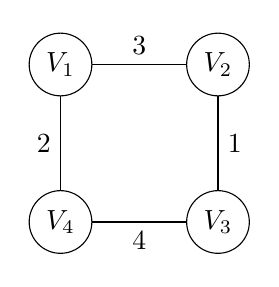
\begin{tikzpicture}
    \node[circle,draw] (V1) at (0,2) {$V_1$};
    \node[circle,draw] (V2) at (2,2) {$V_2$};
    \node[circle,draw] (V3) at (2,0) {$V_3$};
    \node[circle,draw] (V4) at (0,0) {$V_4$};
    \draw (V1) -- (V2) node[midway,above] {3};
    \draw (V1) -- (V4) node[midway,left] {2};
    \draw (V4) -- (V3) node[midway,below] {4};
    \draw (V2) -- (V3) node[midway,right] {1};
\end{tikzpicture}
\end{center}

According to the algorithm,

$ V_{-} S=\left\{v_1, v_2\right) \quad E_{-} S=\left\{\left(v_1, v_2\right)\right\}$

$ V_{-}T=\left\{v_3, v_4\right\} \quad E_{-} T=\left\{\left(v_3, v_4\right)\right\}$

$ \therefore M S T\_S=\left\{\left(v_1, v_2\right)\right\} $, $ M S T\_T=\left\{\left(v_3, v_4\right)\right\}$

$\because$ weight $\left(v_2, v_3\right)=1<$ weight $\left(v_1, v_4\right)=2 $

$e=\left\{\left(v_2, v_3\right)\right\}$

$ \therefore M S T=\left\{\left(v_1, v_2\right),\left(v_3, v_4\right)\left(v_2, v_3\right)\right\}$ will be returned

The weight will be $1+3+4=8$.

But the MST in this graph is $\left\{\left(v_4, v_1\right),\left(v_1, v_2\right),\left(v_2, v_3\right)\right\}$

So the returned one is not a MST
and this algorithm can't guarantee to output a MST.

$\Rightarrow$ The new algorithm is false.

QED.
\end{document}